\section{Results}
\label{sec:results}

\subsection{Accuracy: CoT loses to black boxes and to its own controls}
\label{sec:results:acc}

\tabref{tab:accuracy} reports out-of-fold accuracy for every arm. \cotarm does not match the best
tabular baseline on any task, and the gaps are far outside the pre-declared equivalence margins.
On \taskone, \xgb reaches AUC 0.794 against \cotarm's 0.616 ($\Delta = -0.178$, margin 0.05). On
\taskthree, \tabpfn reaches 0.842 against \cotarm's 0.681 ($\Delta = -0.161$). On \tasktwo, \tabpfn
reaches 5.28\,y MAE against \cotarm's 11.43\,y ($\Delta = +6.15$\,y, margin 1.5\,y)---and every LLM
condition on \tasktwo is worse than the 9.07\,y of simply predicting the cohort mean age. On that
task the LLM arm is not merely behind the baselines; it has negative practical value. The
hypothesis that a reasoning LLM matches black-box accuracy is refuted on all three tasks.

\begin{figure}[t]
    \centering
    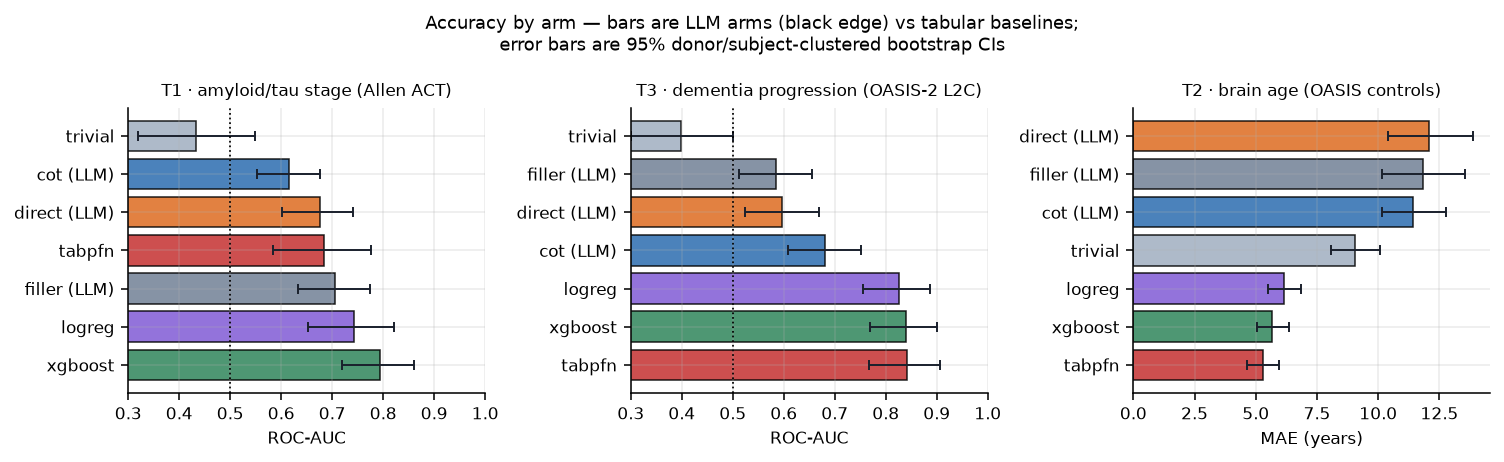
\includegraphics[width=0.95\linewidth]{figures/fig1_accuracy.png}
    \caption{
        Accuracy by arm and family across the three tasks, with donor/subject-clustered bootstrap
        CIs. Tabular arms are consistently above the LLM arms on the two classification tasks, and
        on \tasktwo (right, lower is better) all three LLM conditions sit above the trivial
        mean-age predictor.
    }
    \label{fig:accuracy}
\end{figure}

\begin{table}[t]
    \centering
    \resizebox{\textwidth}{!}{%
    \begin{tabular}{@{}llcc c llcc@{}}
        \toprule
        \multicolumn{4}{c}{\textsc{\taskone} --- Braak $\geq$\,IV (377 samples / 107 donors)} & &
        \multicolumn{4}{c}{\textsc{\taskthree} --- progression (223 predictions / 150 subjects)} \\
        \cmidrule(lr){1-4} \cmidrule(lr){6-9}
        Arm & Family & ROC-AUC [95\% CI] & Bal.\ acc. & & Arm & Family & ROC-AUC [95\% CI] & Bal.\ acc. \\
        \midrule
        \xgb        & tabular & {\bf 0.794} [0.719, 0.860] & 0.698 & & \tabpfn     & tabular & {\bf 0.842} [0.768, 0.907] & {\bf 0.776} \\
        \logreg     & tabular & 0.742 [0.653, 0.821] & 0.640 & & \xgb        & tabular & 0.840 [0.770, 0.900] & 0.737 \\
        \filler     & llm     & 0.706 [0.633, 0.773] & {\bf 0.700} & & \logreg     & tabular & 0.826 [0.756, 0.887] & 0.748 \\
        \tabpfn     & tabular & 0.685 [0.584, 0.776] & 0.632 & & \cotarm        & llm     & 0.681 [0.609, 0.751] & 0.666 \\
        \direct     & llm     & 0.676 [0.601, 0.741] & 0.689 & & \direct     & llm     & 0.597 [0.523, 0.669] & 0.702 \\
        \cotarm        & llm     & 0.616 [0.552, 0.676] & 0.649 & & \filler     & llm     & 0.585 [0.513, 0.654] & 0.684 \\
        \trivial    & tabular & 0.432 [0.320, 0.548] & 0.500 & & \trivial    & tabular & 0.399 [0.299, 0.499] & 0.500 \\
        \bottomrule
    \end{tabular}
    }

    \vspace{6pt}

    \resizebox{0.72\textwidth}{!}{%
    \begin{tabular}{@{}llccc@{}}
        \toprule
        \multicolumn{5}{c}{\textsc{\tasktwo} --- brain age, cognitively normal scans (323 scans / 207 subjects)} \\
        \midrule
        Arm & Family & MAE (years) [95\% CI] & RMSE & Pearson $r$ \\
        \midrule
        \tabpfn  & tabular & {\bf 5.28} [4.65, 5.93] & {\bf 7.01} & {\bf 0.794} \\
        \xgb     & tabular & 5.68 [5.04, 6.34] & 7.38 & 0.771 \\
        \logreg  & tabular & 6.16 [5.51, 6.85] & 7.78 & 0.739 \\
        \trivial & tabular & \emph{9.07} [8.08, 10.09] & \emph{11.63} & \emph{$-0.156$} \\
        \cotarm     & llm     & 11.43 [10.14, 12.79] & 14.61 & 0.277 \\
        \filler  & llm     & 11.82 [10.15, 13.54] & 15.89 & 0.118 \\
        \direct  & llm     & 12.08 [10.39, 13.88] & 16.31 & 0.102 \\
        \bottomrule
    \end{tabular}
    }
    \caption{
        Out-of-fold accuracy under grouped 5-fold cross-validation, with donor/subject-clustered
        bootstrap CIs ($B=2000$). Best per column in {\bf bold}. \cotarm never reaches the best tabular
        baseline on any task, and on \tasktwo \emph{every} LLM condition is worse than the trivial
        predictor that outputs the cohort mean age (italicised).
    }
    \label{tab:accuracy}
\end{table}


\para{Does CoT at least beat its own no-reasoning controls?} \tabref{tab:contrasts} answers with
paired contrasts on identical rows. On \taskone it does not: \cotarm is $0.090$ AUC \emph{below}
compute-matched filler tokens (95\% CI $[-0.156, -0.024]$, $q=0.048$, McNemar $p=0.015$), and
$0.060$ below \direct. Reasoning here is worse than emitting the same number of meaningless tokens.
On \taskthree the sign reverses ($+0.096$ over \filler, $q=0.048$), and on \tasktwo no contrast is
significant.

\para{The \taskthree reversal is mostly a confidence artefact.} Classification AUC is computed from
the model's stated confidence, so confidence granularity is a candidate explanation, and
\tabref{tab:calibration} shows it is the right one. The \direct condition on \taskthree emits only
\emph{two} distinct confidence values, which mechanically caps its AUC. On balanced accuracy, which
does not depend on confidence resolution, \direct is in fact better than \cotarm (0.702 vs.\ 0.666).
What \cotarm genuinely delivers on \taskthree is much better calibration---ECE 0.083 against 0.314 for
\direct and 0.287 for \filler (\figref{fig:calibration}). Communicating uncertainty well is a real
clinical good, but it is a different benefit from the one the interpretability hypothesis predicts.

\begin{table}[t]
    \centering
    \resizebox{\textwidth}{!}{%
    \begin{tabular}{@{}llcrccl@{}}
        \toprule
        Task & Contrast & Metric & Difference [95\% CI] & $p$ (boot) & $q$ (BH) & Paired test \\
        \midrule
        \taskone   & \cotarm $-$ \direct & $\Delta$AUC & $-0.060$ [$-0.127$, $+0.009$] & 0.084 & 0.151 & McNemar $p=0.056$ \\
        \taskone   & \cotarm $-$ \filler & $\Delta$AUC & {\bf $-0.090$} [$-0.156$, $-0.024$] & {\bf 0.010} & {\bf 0.048} & McNemar $p=0.015$ \\
        \taskone   & \direct $-$ \filler & $\Delta$AUC & $-0.030$ [$-0.057$, $-0.006$] & 0.016 & 0.048 & McNemar $p=0.180$ \\
        \midrule
        \taskthree & \cotarm $-$ \direct & $\Delta$AUC & $+0.084$ [$+0.008$, $+0.158$] & 0.029 & 0.065 & McNemar $p=0.615$ \\
        \taskthree & \cotarm $-$ \filler & $\Delta$AUC & {\bf $+0.096$} [$+0.023$, $+0.173$] & {\bf 0.014} & {\bf 0.048} & McNemar $p=1.000$ \\
        \taskthree & \direct $-$ \filler & $\Delta$AUC & $+0.012$ [$-0.045$, $+0.075$] & 0.672 & 0.672 & McNemar $p=0.332$ \\
        \midrule
        \tasktwo   & \cotarm $-$ \direct & $\Delta$MAE & $-0.65$\,y [$-2.18$, $+0.72$] & 0.391 & 0.503 & Wilcoxon $p=0.833$ \\
        \tasktwo   & \cotarm $-$ \filler & $\Delta$MAE & $-0.39$\,y [$-1.82$, $+0.93$] & 0.586 & 0.659 & Wilcoxon $p=0.784$ \\
        \bottomrule
    \end{tabular}
    }
    \caption{
        Paired condition contrasts on identical rows, clustered paired bootstrap with
        Benjamini--Hochberg FDR within family. On \taskone, \cotarm is significantly worse than
        semantically empty filler tokens of the same length. On \taskthree the sign reverses, but
        \tabref{tab:calibration} shows that advantage is largely a confidence-verbalisation effect.
        On \tasktwo no contrast is significant. Negative $\Delta$MAE favours \cotarm.
    }
    \label{tab:contrasts}
\end{table}

\begin{table}[t]
    \centering
    \resizebox{0.85\textwidth}{!}{%
    \begin{tabular}{@{}llccccc@{}}
        \toprule
        Task & Condition & Distinct conf.\ values & Conf.\ entropy & Balanced acc. & ROC-AUC & ECE \\
        \midrule
        \taskthree & \cotarm    & 10 & 1.913 & 0.666 & {\bf 0.681} & {\bf 0.083} \\
        \taskthree & \direct & {\bf 2}  & 0.644 & {\bf 0.702} & 0.597 & 0.314 \\
        \taskthree & \filler & 8  & 1.274 & 0.684 & 0.585 & 0.287 \\
        \midrule
        \taskone   & \cotarm    & 10 & 1.533 & 0.649 & 0.616 & 0.289 \\
        \taskone   & \direct & 8  & 1.189 & 0.689 & 0.676 & 0.305 \\
        \taskone   & \filler & 8  & 1.279 & {\bf 0.706} & {\bf 0.706} & 0.294 \\
        \bottomrule
    \end{tabular}
    }
    \caption{
        A confound we checked rather than assumed. AUC is computed from the model's \emph{stated}
        confidence, so confidence granularity can drive it. On \taskthree the \direct condition
        emits only two distinct confidence values, which mechanically depresses its AUC; on the
        threshold-free metric \direct is in fact better than \cotarm (0.702 vs.\ 0.666). What \cotarm does
        genuinely deliver on \taskthree is far better calibration (ECE 0.083 vs.\ 0.314)---a real
        benefit, but a different one from the hypothesised gain in discrimination.
    }
    \label{tab:calibration}
\end{table}


\begin{figure}[t]
    \centering
    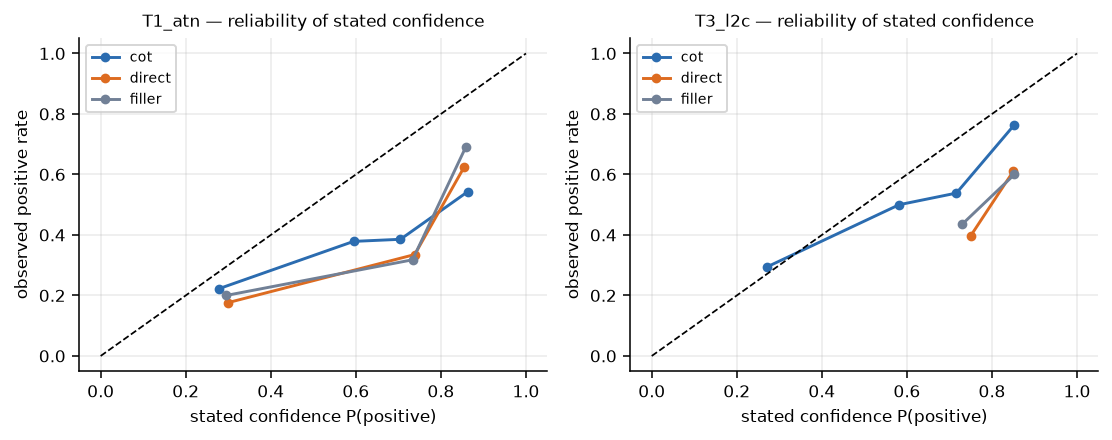
\includegraphics[width=0.9\linewidth]{figures/fig6_calibration.png}
    \caption{
        Confidence resolution and calibration. \cotarm spreads its confidence over ten distinct values
        on both classification tasks, whereas \direct collapses to two on \taskthree. The
        reliability curves show \cotarm is the only well-calibrated condition on \taskthree
        (ECE 0.083), and that all three conditions are similarly overconfident on \taskone.
    }
    \label{fig:calibration}
\end{figure}

\subsection{Faithfulness: the chains are not doing the work}
\label{sec:results:faith}

\tabref{tab:faithfulness} and \figref{fig:early} report the intervention battery. On \taskone,
showing the model \emph{none} of its own reasoning and forcing an answer reproduces the full-chain
answer 82.9\% of the time; the early-answering curve is nearly flat, giving
$\aoc = 0.066$ $[0.042, 0.093]$. Corrupting a biomarker value inside the chain by a factor of ten
changes the final answer 3.6\% of the time $[0.000, 0.079]$. \taskthree is similar (agreement 0.757,
$\aoc = 0.090$, mistake sensitivity 0.022). On these tasks the chain is post-hoc narration of an
answer that already exists.

Paraphrase sensitivity is uniformly low (1.4--5.6\%), which rules out the alternative explanation
that the chains carry information in an encoded or steganographic form. The information is where it
appears to be; there is simply very little of it.

\para{Regression inverts the picture.} On \tasktwo, \aoc is 0.378 $[0.335, 0.425]$---5.7$\times$
higher than \taskone---and mistake injection moves the prediction by 0.33\,SD. The chain is
genuinely load-bearing when the target is continuous. To our knowledge this is the first evidence
that CoT faithfulness differs systematically between classification and regression, and it runs
opposite to the accuracy numbers, since \tasktwo is the task the LLM performs worst on. The
plausible mechanism is that a two-way choice can be produced in a single forward pass and then
narrated, whereas producing a specific number appears to require the intermediate arithmetic-like
steps to actually be written.

\begin{figure}[t]
    \centering
    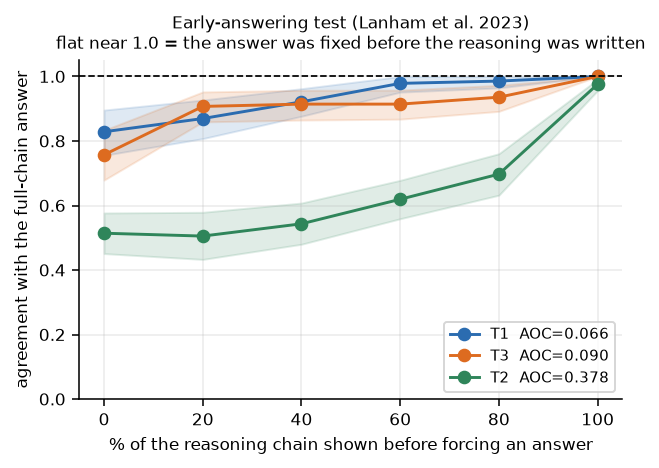
\includegraphics[width=0.95\linewidth]{figures/fig2_early_answering.png}
    \caption{
        Early answering. Each curve shows how often the answer produced from a truncated chain
        matches the full-chain answer, as a function of how much of the chain the model is shown.
        A faithful chain should start low and climb; the two classification tasks start at
        0.76--0.83, meaning the answer is essentially fixed before any reasoning is revealed. The
        continuous target (\tasktwo, using the normalised answer shift of \eqref{eq:shift}) is the
        only task with a substantial area over the curve.
    }
    \label{fig:early}
\end{figure}

\begin{table}[t]
    \centering
    \resizebox{0.9\textwidth}{!}{%
    \begin{tabular}{@{}lccc@{}}
        \toprule
        Metric & \textsc{\taskone} (classif.) & \textsc{\taskthree} (classif.) & \textsc{\tasktwo} (regression) \\
        \midrule
        Agreement with full-chain answer at 0\% of chain shown & 0.829 & 0.757 & 0.514 \\
        Early-answering \aoc [95\% CI] & {\bf 0.066} [0.042, 0.093] & 0.090 [0.058, 0.126] & {\bf 0.378} [0.335, 0.425] \\
        Mistake-injection answer-change rate [95\% CI] & {\bf 0.036} [0.000, 0.079] & 0.022 [0.000, 0.056] & {\bf 0.325} [0.238, 0.428] \\
        Paraphrase answer-change rate [95\% CI] & 0.014 [0.000, 0.037] & 0.021 [0.000, 0.049] & 0.056 [0.031, 0.084] \\
        \bottomrule
    \end{tabular}
    }
    \caption{
        Causal faithfulness of the \qwenseven chains. On the two classification tasks the chains are
        essentially post-hoc narration: showing the model none of its own reasoning reproduces the
        full-chain answer 75--83\% of the time, and a 10$\times$ corruption of a biomarker value
        inside the chain changes the answer 2--4\% of the time. On the continuous target the picture
        inverts---\aoc is 5.7$\times$ higher and mistake injection moves the prediction by 0.33\,SD.
        Uniformly low paraphrase sensitivity shows the chains are not using encoded reasoning; the
        information is where it appears to be, there is simply very little of it.
    }
    \label{tab:faithfulness}
\end{table}


\subsection{\cfit and \esa}
\label{sec:results:cfit}

\tabref{tab:cfit_esa} reports the two new metrics. \cfit is positive: perturbing the features a
chain names as decisive shifts its prediction 1.39$\times$ (\taskone), 2.13$\times$ (\taskthree,
$p=0.0005$) and 1.54$\times$ (\tasktwo, $p=0.007$) more than perturbing an equal-sized random set of
features the chain ignores. This is the one clear positive for CoT-as-interpretability: even when
the global chain is post-hoc, the specific measurements it points at do carry causal weight. Because
our citation parser is a deliberately conservative lexical matcher, paraphrastic citations are
undercounted and this estimate is biased toward the null.

\esa is negative on the primary task. Citation frequency and permutation importance are essentially
uncorrelated on \taskone ($\rho = 0.126$, $p = 0.629$) and \tasktwo ($\rho = 0.105$, $p = 0.895$),
and only modestly aligned on \taskthree ($\rho = 0.491$, $p = 0.039$). The reason is visible in
\figref{fig:esa}: the chains cite nearly every biomarker in nearly every case---total tau and pTau at
a 100\% rate, AT8 at 98.6\%---so citation frequency carries almost no information about which
biomarker matters. The chains \emph{do} mention AT8, the single decisive feature by permutation
importance ($\Delta$AUC 0.110, four times the next feature); they simply mention it no more than
they mention uninformative ones. An explanation that names everything explains nothing.

\begin{table}[t]
    \centering
    \begin{minipage}{0.49\textwidth}
    \centering
    \resizebox{\textwidth}{!}{%
    \begin{tabular}{@{}lcccc@{}}
        \toprule
        Task & Cited & Uncited & Ratio & $p$ (boot) \\
        \midrule
        \taskone   & 0.279 & 0.200 & 1.39$\times$ & 0.090 \\
        \taskthree & 0.364 & 0.171 & {\bf 2.13$\times$} & {\bf 0.0005} \\
        \tasktwo   & 0.669 & 0.434 & {\bf 1.54$\times$} & {\bf 0.007} \\
        \bottomrule
    \end{tabular}
    }
    \subcaption{\cfit: normalised prediction shift when the features a chain names as decisive are
    perturbed by $\pm1$\,SD, versus an equal-sized random set it ignores.}
    \label{tab:cfit}
    \end{minipage}
    \hfill
    \begin{minipage}{0.49\textwidth}
    \centering
    \resizebox{\textwidth}{!}{%
    \begin{tabular}{@{}lccl@{}}
        \toprule
        Task & Spearman $\rho$ & $p$ & Highest-signal feature \\
        \midrule
        \taskone   & 0.126 & 0.629 & AT8 ($\Delta$AUC 0.110) \\
        \taskthree & {\bf 0.491} & {\bf 0.039} & lowest-ever MMSE (0.126) \\
        \tasktwo   & 0.105 & 0.895 & nWBV (6.39\,y) \\
        \bottomrule
    \end{tabular}
    }
    \subcaption{\esa: rank correlation between per-feature citation frequency and permutation
    importance measured independently on the black-box arm.}
    \label{tab:esa}
    \end{minipage}
    \caption{
        The two new interpretability metrics. \cfit is the one clear positive for
        CoT-as-interpretability: the measurements a chain points at are more influential than the
        ones it passes over, significantly so on \taskthree and \tasktwo. \esa is negative on the
        primary task---the chains cite total tau and pTau in 100\% of cases and AT8 in 98.6\%, so
        citation frequency carries almost no information about which biomarker matters. An
        explanation that names everything explains nothing.
    }
    \label{tab:cfit_esa}
\end{table}


\begin{figure}[t]
    \centering
    \begin{subfigure}[b]{0.48\textwidth}
        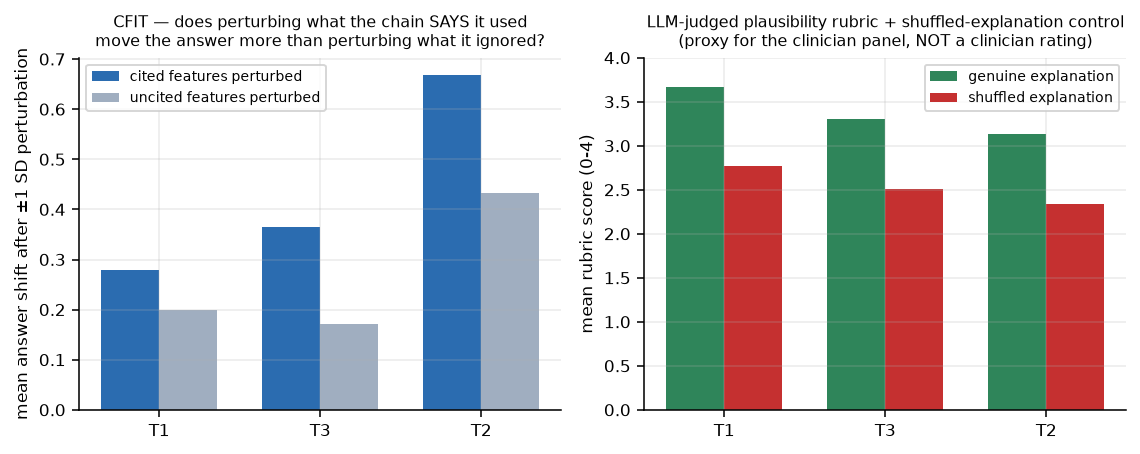
\includegraphics[width=\textwidth]{figures/fig4_cfit_judge.png}
        \caption{\cfit and blinded rubric}
        \label{fig:cfit}
    \end{subfigure}
    \hfill
    \begin{subfigure}[b]{0.48\textwidth}
        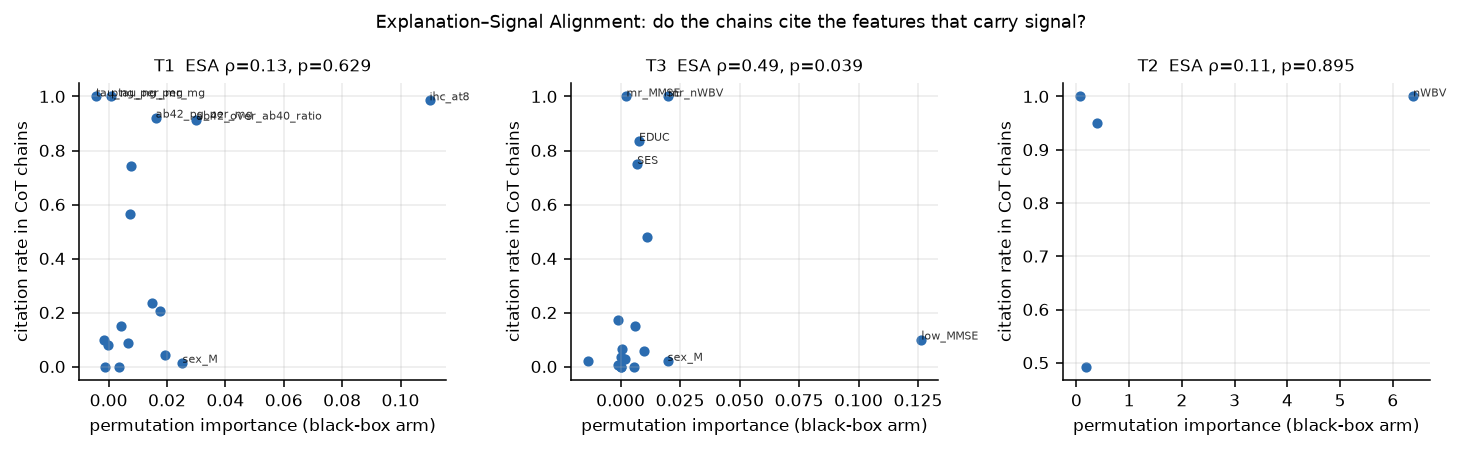
\includegraphics[width=\textwidth]{figures/fig5_esa.png}
        \caption{\esa}
        \label{fig:esa}
    \end{subfigure}
    \caption{
        \captiona \cfit shift for cited versus uncited features, alongside blinded rubric scores for
        genuine and shuffled rationales. \captionb Per-feature citation frequency against
        independently measured permutation importance. The chains saturate their citations---most
        features are named in most cases---so the ranking carries little signal on \taskone.
    }
    \label{fig:cfit_esa}
\end{figure}

\subsection{Robustness: supported in slope, vacuous in level}
\label{sec:results:robust}

\tabref{tab:robustness} and \figref{fig:robustness} report the perturbation sweeps. The \cotarm arm is
essentially flat under missingness on \taskone ($+2.4\%$ from clean to 50\% MCAR) and \tasktwo
($-4.0\%$, \ie slightly better), while \xgb loses 20.6\% of its AUC on \taskone and more than
doubles its MAE on \tasktwo. This matches the observation of \citet{kearney2026tapgpt} that LLM
prompts represent missingness natively and require no imputation.

But flatness is not an advantage when the level is low. On \taskone, \cotarm at 50\% missingness (0.609)
is still below \xgb at 50\% missingness (0.630). On \tasktwo the crossover is real and quantitative:
\xgb degrades past the \cotarm arm somewhere between 20\% and 30\% missingness and reaches 14.23\,y at
50\% against \cotarm's 10.83\,y. \tabpfn, however, stays better than the LLM at every level tested
(8.01\,y at 50\% MCAR). The actionable conclusion is therefore about tabular foundation models, not
about reasoning. And on \taskthree the pattern does not hold at all: \cotarm is the \emph{least} robust
arm ($-22.2\%$), worse than every tabular baseline.

\begin{figure}[t]
    \centering
    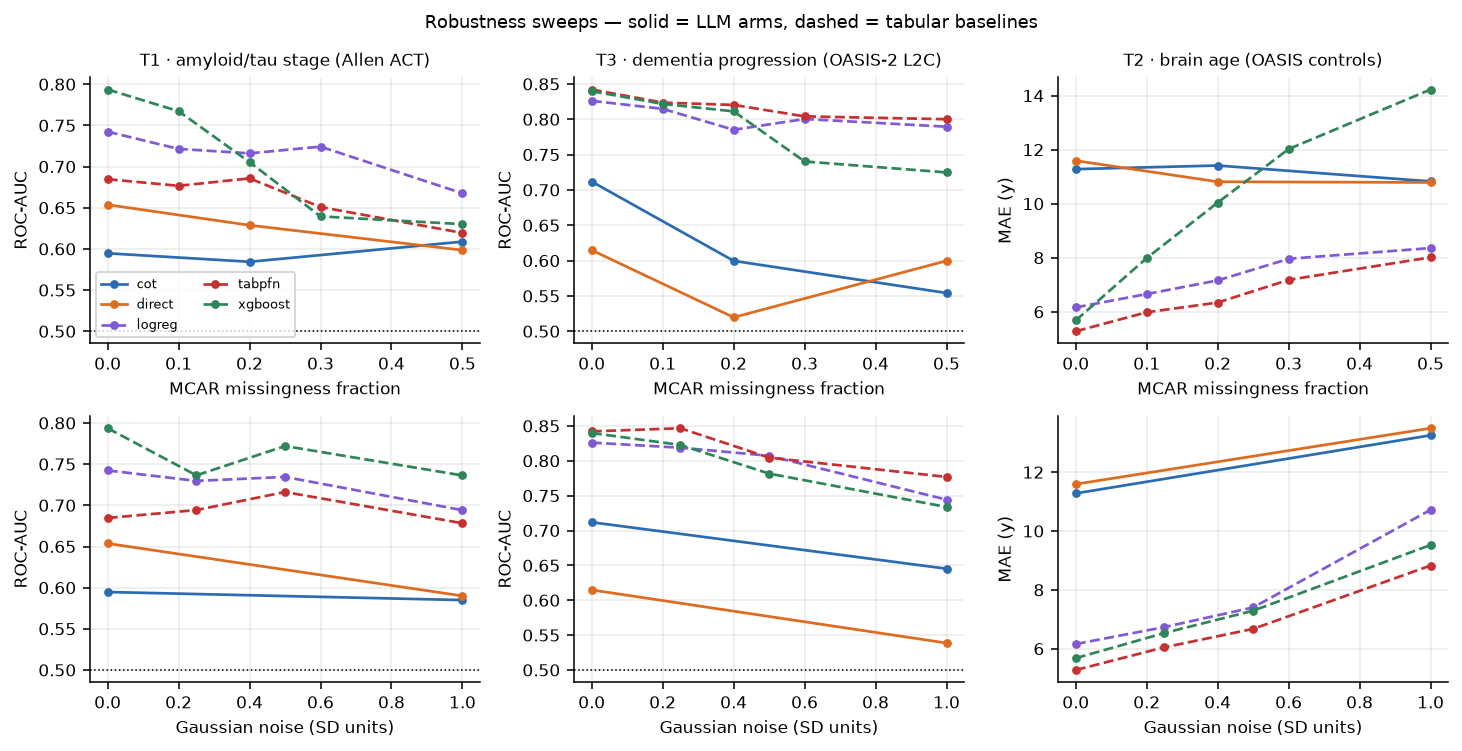
\includegraphics[width=0.95\linewidth]{figures/fig3_robustness.png}
    \caption{
        Performance under MCAR missingness and Gaussian feature noise, with every arm receiving the
        same corrupted values. The LLM curves are nearly horizontal, but they are horizontal at a
        level the tabular baselines only reach under extreme corruption. \tabpfn dominates the LLM
        arm at every perturbation level on \tasktwo.
    }
    \label{fig:robustness}
\end{figure}

\begin{table}[t]
    \centering
    \resizebox{0.8\textwidth}{!}{%
    \begin{tabular}{@{}llccr@{}}
        \toprule
        Task & Arm & Clean & 50\% MCAR & Relative change \\
        \midrule
        \taskone   & \xgb    & 0.794 & 0.630 & $-20.6\%$ \\
        \taskone   & \logreg & 0.742 & 0.668 & $-10.1\%$ \\
        \taskone   & \cotarm    & 0.595 & 0.609 & {\bf $+2.4\%$} \\
        \taskone   & \direct & 0.654 & 0.599 & $-8.4\%$ \\
        \midrule
        \taskthree & \xgb    & 0.840 & 0.725 & $-13.7\%$ \\
        \taskthree & \tabpfn & 0.842 & 0.800 & {\bf $-5.0\%$} \\
        \taskthree & \cotarm    & 0.712 & 0.554 & $-22.2\%$ \\
        \midrule
        \tasktwo   & \xgb    & 5.68\,y & 14.23\,y & $+150.5\%$ (worse) \\
        \tasktwo   & \tabpfn & 5.28\,y & 8.01\,y & $+51.9\%$ (worse) \\
        \tasktwo   & \cotarm    & 11.28\,y & 10.83\,y & {\bf $-4.0\%$} (better) \\
        \bottomrule
    \end{tabular}
    }
    \caption{
        Degradation from clean data to 50\% MCAR missingness (AUC for \taskone/\taskthree, MAE for
        \tasktwo). The \cotarm arm is essentially flat under missingness on \taskone and \tasktwo---but
        flat at a level the baselines only fall \emph{to} under extreme corruption. On \taskthree it
        is the least robust arm of all. The robustness claim is supported in slope and vacuous in
        level.
    }
    \label{tab:robustness}
\end{table}


\subsection{The clinical endpoint: a brain-age gap with no disease signal}
\label{sec:results:bag}

A brain-age model is clinically interesting only if the gap between predicted and chronological age
tracks disease. \tabref{tab:brainage} compares the age-bias-corrected gap between out-of-fold
controls and demented scans. The conventional models reproduce the textbook finding of roughly four
years of apparent brain ageing in dementia ($+4.26$\,y for \tabpfn, Cohen's $d = 0.730$,
AUC 0.701). The \cotarm-derived gap is $+0.15$\,y, with AUC 0.490 $[0.435, 0.547]$ and $p = 0.670$: no
disease signal whatsoever. This is the most clinically legible result in the study. The reasoning
chains are articulate about atrophy and ageing, and the quantity they produce is diagnostically
empty.

\begin{table}[t]
    \centering
    \resizebox{0.85\textwidth}{!}{%
    \begin{tabular}{@{}llccccc@{}}
        \toprule
        Arm & Family & \bag in demented & \bag in controls & ROC-AUC [95\% CI] & Cohen's $d$ & $p$ \\
        \midrule
        \tabpfn & tabular & {\bf $+4.26$\,y} & 0.00 & {\bf 0.701} [0.646, 0.757] & {\bf 0.730} & $<10^{-4}$ \\
        \logreg & tabular & $+3.90$\,y & 0.00 & 0.691 [0.633, 0.749] & 0.660 & $<10^{-4}$ \\
        \xgb    & tabular & $+4.10$\,y & 0.00 & 0.683 [0.628, 0.737] & 0.664 & $<10^{-4}$ \\
        \midrule
        \cotarm    & llm     & $+0.15$\,y & 0.00 & 0.490 [0.435, 0.547] & 0.015 & 0.670 \\
        \direct & llm     & $-0.20$\,y & 0.00 & 0.470 [0.408, 0.535] & $-0.019$ & 0.202 \\
        \bottomrule
    \end{tabular}
    }
    \caption{
        The clinical endpoint. Normative models are fitted on cognitively normal scans only and the
        regression-to-the-mean bias is removed within controls, so the control gap is zero by
        construction. The conventional models reproduce the textbook finding of roughly four years
        of apparent brain ageing in dementia; the \cotarm-derived gap carries no disease signal at all
        (AUC 0.490, $p=0.670$). The chains are articulate about atrophy and ageing, and the quantity
        they produce is diagnostically empty.
    }
    \label{tab:brainage}
\end{table}


\subsection{Blinded plausibility: persuasive in proportion to how little it does}
\label{sec:results:judge}

\tabref{tab:judge} reports the blinded rubric. The shuffled-explanation control passes on all three
tasks---genuine rationales score 0.79--0.90 points above rationales written for a different patient,
with $p < 10^{-23}$---so the rubric discriminates rather than rubber-stamping. Given that validity
check, the headline is the dissociation. On \taskone the chains score 3.67/4 overall, including
4.00/4 for absence of fabrication and 3.96/4 for biological validity, while responding to a
10$\times$ corruption of their own content 3.6\% of the time. The chains are rated as
near-perfectly non-fabricating and biologically sound while being almost entirely disconnected from
the computation that produced the answer. We note that these are LLM-proxy scores produced by the
same base model that generated the chains, which risks self-preference; see \secref{sec:discussion}.

\begin{table}[t]
    \centering
    \resizebox{0.8\textwidth}{!}{%
    \begin{tabular}{@{}lccccc@{}}
        \toprule
        Task & Genuine explanation & Shuffled (mismatched) & Difference & Mann--Whitney $p$ & Mistake sensitivity \\
        \midrule
        \taskone   & {\bf 3.67}\,/\,4 & 2.78 & $+0.90$ & $9.7\times10^{-24}$ & 0.036 \\
        \taskthree & 3.30\,/\,4 & 2.51 & $+0.79$ & $1.0\times10^{-31}$ & 0.022 \\
        \tasktwo   & 3.13\,/\,4 & 2.34 & $+0.79$ & $5.7\times10^{-31}$ & 0.325 \\
        \bottomrule
    \end{tabular}
    }
    \caption{
        The dissociation. The shuffled-explanation control passes---the rubric reliably separates a
        genuine rationale from one written for a different patient---so the scores are
        discriminative rather than a rubber stamp. Given that, the headline is that \taskone chains
        score 3.67/4 for plausibility while responding to a 10$\times$ corruption of their own
        content 3.6\% of the time. Scores are LLM-proxy ratings, not clinician ratings.
    }
    \label{tab:judge}
\end{table}


\subsection{Model size: CoT is faithful exactly where it is needed}
\label{sec:results:size}

\tabref{tab:modelsize} and \figref{fig:modelsize} report the cleanest causal story in the study, with
accuracy and faithfulness reported jointly as \citet{bentham2024disguised} require. \qwensmall
cannot do \taskone without reasoning: its \direct AUC is 0.504, indistinguishable from chance. CoT
lifts it to 0.586 ($\Delta$AUC $+0.082$ $[+0.018, +0.143]$, $p=0.012$), and its chains are
correspondingly load-bearing---\aoc 0.246 against the 7B model's 0.066 (3.7$\times$) and mistake
sensitivity 0.218 against 0.036 (6$\times$). \qwenseven already knows the answer without reasoning
(\direct AUC 0.676); its chains are decorative, and making it verbalise them costs 0.060 AUC.

CoT is faithful exactly where the model needs it to compute, and decorative exactly where it does
not. This is precisely backwards from the deployment incentive: a clinical system would deploy the
larger, more accurate model, and would therefore get the least trustworthy explanations.

\begin{figure}[t]
    \centering
    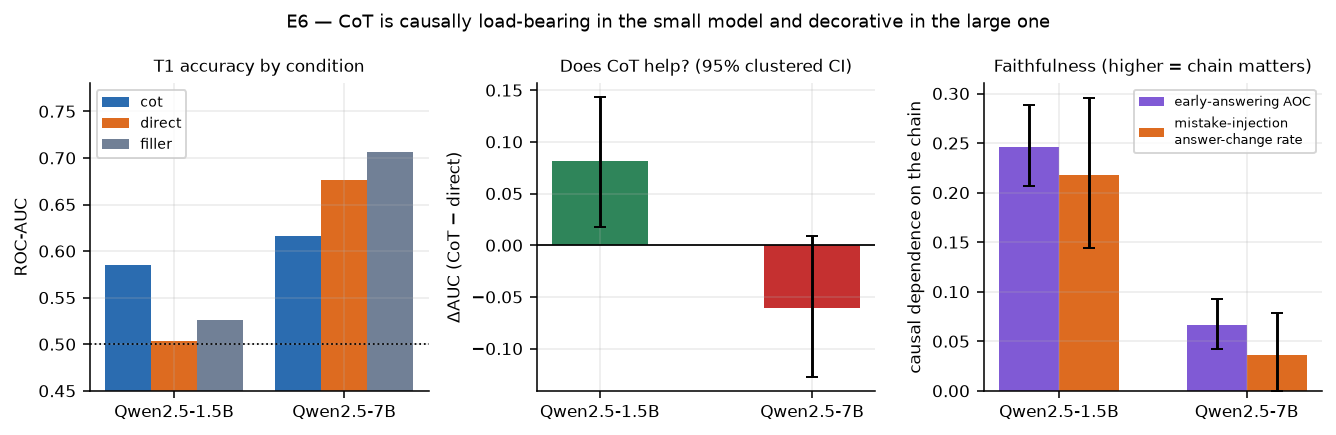
\includegraphics[width=0.9\linewidth]{figures/fig7_model_size.png}
    \caption{
        Accuracy benefit of CoT and causal faithfulness of the resulting chains, for \qwensmall and
        \qwenseven on \taskone. Both move together, and both move \emph{down} with capability: the
        smaller model gains from reasoning and reasons faithfully, the larger model loses from
        reasoning and narrates.
    }
    \label{fig:modelsize}
\end{figure}

\begin{table}[t]
    \centering
    \resizebox{0.8\textwidth}{!}{%
    \begin{tabular}{@{}lcc@{}}
        \toprule
        Quantity (\taskone) & \qwensmall & \qwenseven \\
        \midrule
        ROC-AUC, \direct & 0.504 & {\bf 0.676} \\
        ROC-AUC, \filler & 0.526 & {\bf 0.706} \\
        ROC-AUC, \cotarm    & 0.586 & 0.616 \\
        $\Delta$AUC (\cotarm $-$ \direct) & {\bf $+0.082$} [$+0.018$, $+0.143$], $p=0.012$ & $-0.060$ [$-0.127$, $+0.009$], $p=0.084$ \\
        \midrule
        Early-answering \aoc & {\bf 0.246} [0.206, 0.289] & 0.066 [0.042, 0.093] \\
        Mistake-injection change rate & {\bf 0.218} [0.144, 0.296] & 0.036 [0.000, 0.079] \\
        Paraphrase change rate & 0.079 & 0.014 \\
        \midrule
        Median chain length (chars) & 1414 & 642 \\
        Forced-answer rate (chain over-ran budget) & 0.456 & 0.000 \\
        \bottomrule
    \end{tabular}
    }
    \caption{
        Accuracy and faithfulness reported jointly, as \citet{bentham2024disguised} require. The
        1.5B model cannot do the task without reasoning (\direct AUC 0.504 $\approx$ chance), CoT
        lifts it to 0.586, and its chains are 3.7$\times$ more causally load-bearing and 6$\times$
        more sensitive to injected mistakes. The 7B model already knows the answer, its chains are
        decorative, and verbalising them costs accuracy. The 1.5B forced-answer rate is a caveat
        on the magnitude, not the direction (\secref{sec:discussion}).
    }
    \label{tab:modelsize}
\end{table}


\subsection{Error analysis}
\label{sec:results:errors}

\para{Reasoning past the decisive biomarker (\taskone).} In the first \cotarm error on \taskone (truth:
early tau; predicted: advanced tau, confidence 85), the chain reads: ``The Abeta-42/40 ratio is high
(4.575), indicating significant amyloid burden. High total tau (1.67 ng/mg) and phospho-tau (1.689
ng/mg) suggest active tau pathology\ldots{} \emph{The AT8 pTau immunoreactivity is minimal, but} the
overall tau burden and the presence of amyloid plaques suggest a more advanced stage of
neurofibrillary tangles.'' AT8 immunoreactivity is the single most informative feature on this task.
The chain notices it, explicitly flags it as minimal, and then overrides it with weaker evidence.
This is the \esa result made concrete: right facts, wrong weighting.

\para{Plausible, well-hedged and wrong (\taskthree).} ``The recent MMSE score of 27 is within normal
limits\ldots{} nWBV at 0.806 is close to the average\ldots{} Given the lack of significant changes
in MMSE and nWBV, and the absence of other markers of neurodegeneration like amyloid or tau
pathology (which are not provided), the risk of dementia is low.'' Truth: demented. A systematic
bias accompanies this: on \taskthree the \cotarm arm predicts dementia in only 29.1\% of cases against
a base rate of 47.1\%, \ie it under-calls progression---the clinically costlier direction of error.

\para{Longer chains do not rescue harder cases.} Chain length is negatively associated with
correctness: point-biserial $r = -0.114$ ($p = 0.027$) on \taskone and $r = -0.178$ ($p = 0.008$) on
\taskthree.

\para{Parsing integrity.} Final answer-parse success was 100.0\% for \qwenseven on all three tasks
and 99.5\% for \qwensmall, so no result depends on discarded generations. Where a generation failed
to emit an answer it was re-run with a forced continuation rather than dropped; the fraction
requiring that was 0.00\%, 0.00\% and 0.19\% for \qwenseven on \taskone/\tasktwo/\taskthree, against
45.6\% for the \qwensmall \cotarm condition, which frequently exceeded the 512-token budget.
